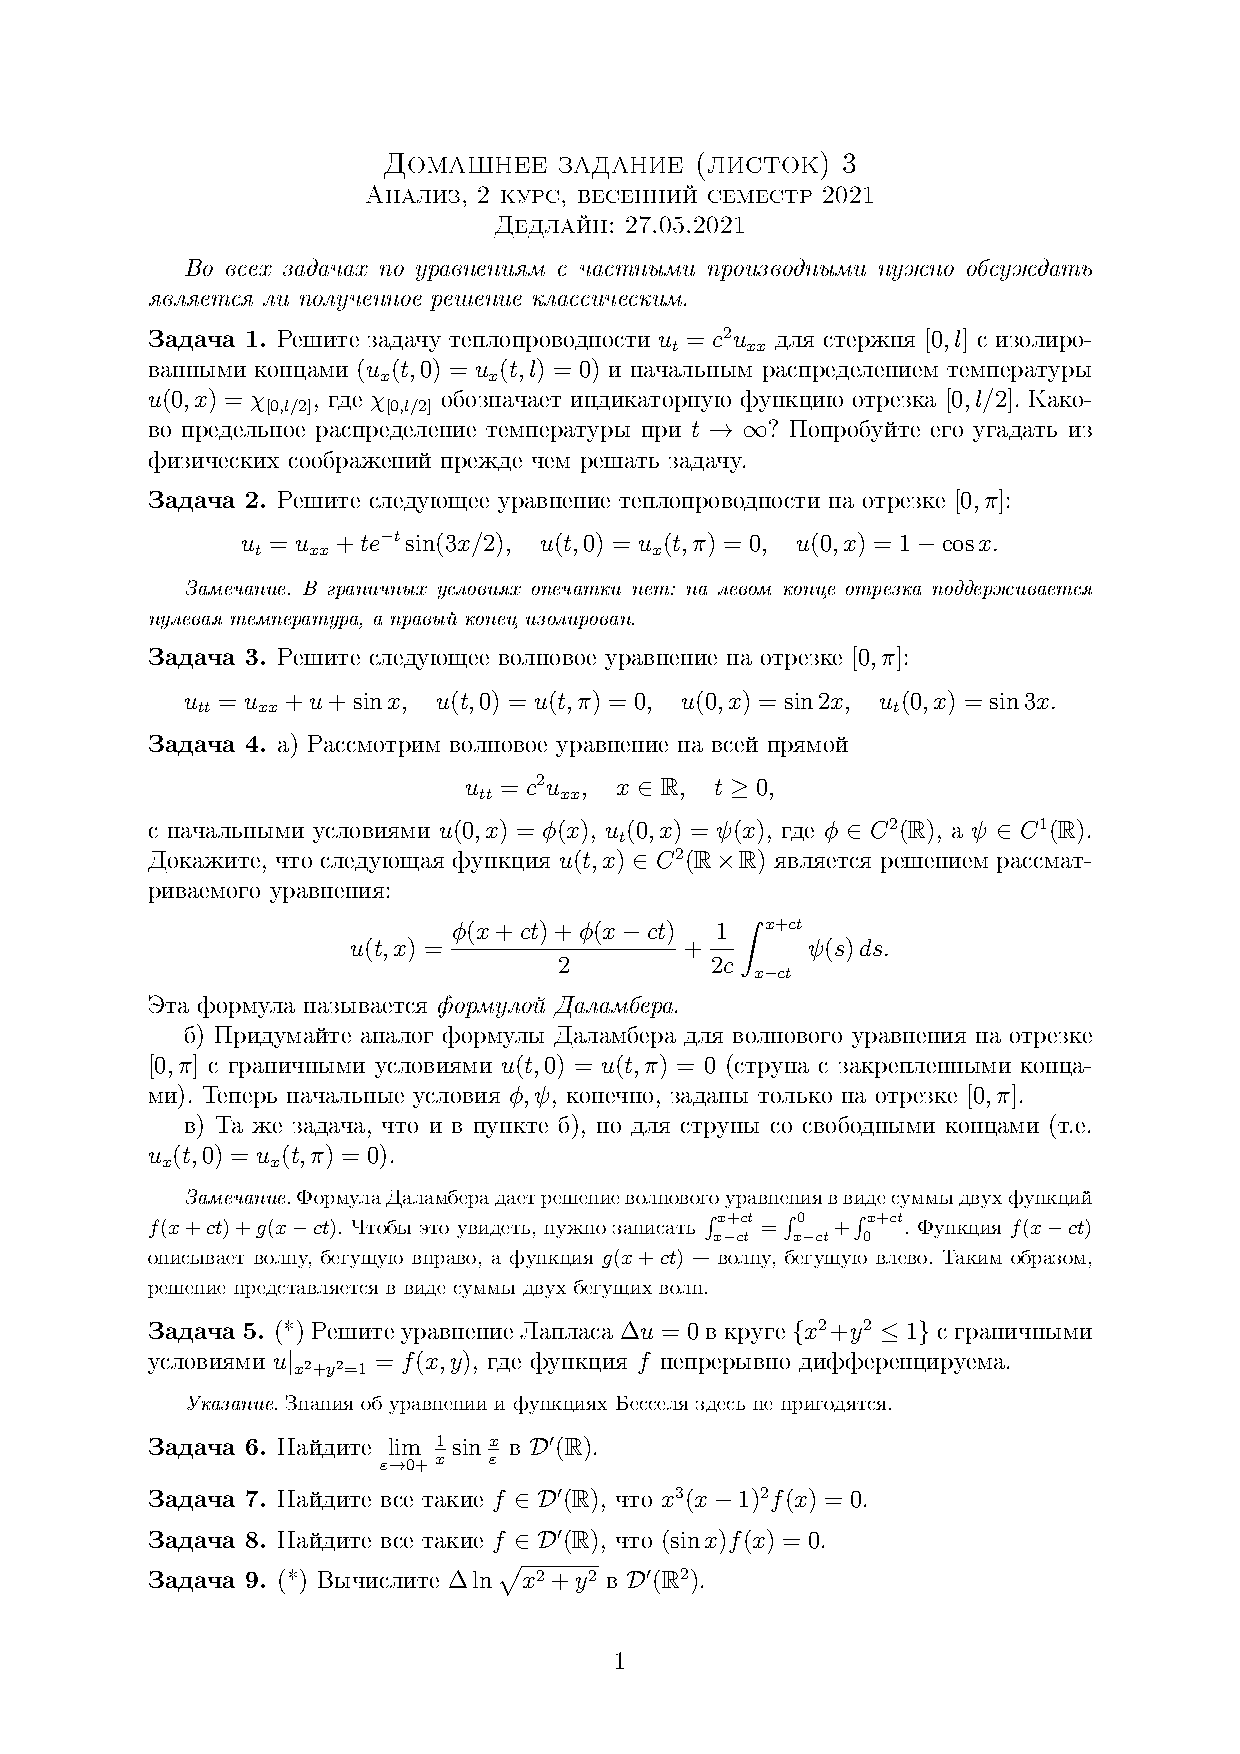
\includepdf[scale=1,pages=1]{Tasks/Listok3_2021.pdf}
\newpage
\section*{Решения}
\subsection*{Задача 1}
	Ищем решения в виде (метод Фурье)
	\begin{equation*}
		u(t,x) = z(t)y(x)
	\end{equation*}
	Подставим в $u_{t} = c^2 u_{xx}$
	\begin{gather*}
		z'(t)y(x) = c^2 z(t) y''(x)\\
		\frac{z'(t)}{z(t)c^2} = \frac{y''(x)}{y(x)} = \lambda
	\end{gather*}
	задача Ш.-Л. $\lambda = -\mu^2$
	\begin{gather*}
		y(x) = A \sin(\mu x) + B \cos(\mu x)\\
		y'(0) = y'(l) = 0\\
		A = 0,\ \mu = \frac{k \pi}{l}\\
		y(x) = B \cos \frac{k \pi}{l} x\\
		z'(t) = \lambda c^2 z(t) = -\left(\frac{k \pi c}{l}\right)^2 z(t)\\
		z(t) = C_{kl}^{-\left(\frac{k \pi c}{l}\right)^2 t}\\
		U(t,x) = \sum A_{k,l}^{-\left(\frac{k \pi c}{l}\right)^2 t} \cos \left(\frac{k \pi}{l}x\right)
	\end{gather*}
	Подставим в $u(0,x) = \chi_{[0,l/2]}$
	\begin{equation*}
		u(0,x) = \sum A_{k} \cos \frac{k \pi}{l} x = \chi_{[0,l/2]} =
		\begin{cases}
			1,\ x \in \left[0, \frac{l}{2}\right]\\
			0,\ \text{иначе}
		\end{cases}
	\end{equation*}
	Раскладываем $\chi_{[0,l/2]}$ в ряд Фурье
	\begin{gather*}
		A_{k} = \frac{\int\limits_{0}^{l} \chi_{[0,l/2]} \cos\left(\frac{k \pi}{l} x\right) dx}{\int\limits_{0}^{l} \cos^2 \left(\frac{k \pi}{l} x\right) dx}\\
		\int\limits_{0}^{l} \cos^2 \left(\frac{k \pi}{l} x\right) dx
		= \int\limits_{0}^{l} \frac{1}{2} + \frac{\cos\left(\frac{2\pi k x}{l}\right)}{2} dx
		= \frac{1}{2}l + \sin \left(\frac{2\pi k x}{l}\right) \frac{l}{2 \pi k \cdot 2} \Big|_{0}^{l}
		= \frac{1}{2}l\\
		\int\limits_{0}^{l} \chi_{[0,l/2]} \cos\left(\frac{k\pi}{l}x\right) dx
		= \int\limits_{0}^{l/2} \cos\left(\frac{k \pi}{l} x\right) dx
		= \frac{l}{\pi k} \sin\left(\frac{k \pi x}{l}\right)\Big|_{0}^{l/2}
		= \frac{l}{\pi k} \sin \frac{k \pi}{2}
		=
		\begin{cases}
			0,\ k = 2n\\
			\frac{l}{\pi k},\ k = 4n+1\\
			-\frac{l}{\pi k},\ k = 4n+3
		\end{cases}\\
		A_{k} =
		\begin{cases}
			0,\ k = 2n\\
			\frac{2}{\pi k},\ k = 4n+1\\
			-\frac{2}{\pi k},\ k = 4n+3
		\end{cases}\\
		u(t,x) =
		\sum\limits_{n = 0}^{\infty} \frac{2}{\pi (4n+1)} e^{-\left(\frac{(4n+1)\pi c}{l}\right)^2 t} \cos \frac{(4n+1)\pi}{l} x +
		\sum\limits_{n = 0}^{\infty} \frac{2}{\pi (4n+3)} e^{-\left(\frac{(4n+3)\pi c}{l}\right)^2 t} \cos \frac{(4n+3)\pi}{l} x
	\end{gather*}
\vskip 0.4in

\subsection*{Задача 2}
	\begin{gather*}
		u(x,t) = y(x)z(t)\\
		u_{t} = u_{xx}\\
		y(x) z'(t) = y''(x) z(t)\\
		\frac{z'(t)}{z(t)} = \frac{y''(x)}{y(x)} = \lambda = -\mu^2\\
		y(x) = A \sin \mu x + B \cos \mu x\\
		u(t,0) = 0 \Rightarrow B = 0\\
		u_{x}(t,\pi) = 0 \Rightarrow \mu A \cos \mu \pi = 0 \Rightarrow \mu_{k} = \frac{1}{2} + k
	\end{gather*}
	Решение задачи будем искать в виде ряда Фурье
	\begin{equation*}
		u(t,x) = \sum u_{k}(t)\sin\left(\left(\frac{1}{2} + k\right)x\right)
	\end{equation*}
	Подставим в $u_{t} = u_{xx} + t e^{-t} \sin(3x/2)$
	\begin{gather*}
		k \ne 1\\
		u'_{k}(t) = -\mu_{k}^{2} u_{k}(t) \Rightarrow u_{k}(t) = c_{k} e^{-\mu^{2}_{k}}\\
		k = 1\\
		u'_{1}(t) = -\frac{9}{4} u_{1}(t) + te^{-t}\\
		u_{1}(t) = c_{1} e^{-\mu_{1}^{2} t} + \frac{4}{5} e^{-t} \left(t - \frac{4}{5}\right)
		= c_{1} e^{-\frac{9}{4}t} + \frac{4}{5} e^{-t}\left(t - \frac{4}{5}\right)\\
		u(t,x) = \left(c_{1} e^{-\frac{9}{4}t} + \frac{4}{5} e^{-t} \left(t - \frac{4}{5}\right)\right) \sin \frac{3x}{2} + \sum\limits_{k = 0,\ k \geqslant 2} c_{k} e^{-\mu_{k}^{2}t} \sin \left(\left(\frac{1}{2}+k\right)x\right)\\
		u(0,x) = (c_{1} - \frac{16}{25}) \sin \frac{3x}{2} + \sum\limits_{k = 0,\ k \geqslant 2} c_{k} \sin \left(\left(\frac{1}{2}+k\right)x\right) = 1 - \cos(x)
	\end{gather*}
	Разложим $1-\cos(x)$ по $\sin \mu_{k} x$
	\begin{gather*}
		1 - \cos(x) = \sum\limits_{k = 0}^{\infty} f_{k} \sin \mu_{k} x\\
		f_{k} = \frac{\int\limits_{0}^{\pi} (1 - \cos(x)) \sin \left(\left(\frac{1+2k}{2}\right)x\right)dx}{\int\limits_{0}^{\pi} \left(\left(\frac{1+2k}{2}\right)x\right)dx}\\
		\int\limits_{0}^{\pi} \frac{1 - \cos((1+2k)x)}{2}dx
		= \frac{1}{2} \pi - \frac{\sin((1+2k)\pi)}{2(1+2k)} = \frac{1}{2}\pi\\
		\int\limits_{0}^{\pi} \sin \left(\frac{1+2k}{2}x\right)dx
		= -\frac{2}{1+2k} \cos\left(\frac{1+2k}{2}x\right)\Big|_{0}^{\pi} = \frac{2}{1+2k}\\
		-\int\limits_{0}^{\pi} \cos(x) \sin \left(\frac{1+2k}{2}x\right)dx
		= -\frac{1}{2} \int\limits_{0}^{\pi} \sin(kx - \frac{1}{2}x) + \sin(kx + \frac{3}{2}x)dx\\
		= \frac{1}{2}\left(\frac{1}{k - \frac{1}{2}} \cos((k - \frac{1}{2})x\right)\Big|_{0}^{\pi} + \frac{1}{k + \frac{3}{2}} \cos ((k + \frac{3}{2})x)\Big|_{0}^{\pi}\\
		= \frac{1}{2} \left(\frac{2}{2k-1}(-1) + \frac{2}{2k+3}(-1)\right)
		= -\frac{1}{2k-1} - \frac{1}{2k+3}
		= -\frac{4k+2}{(4k^2 + 4k - 3)}
	\end{gather*}
	\begin{gather*}
		f_{k} = \frac{\int\limits_{0}^{\pi}(1-\cos(x))\sin\left(\left(\frac{1+2k}{2}\right)x\right)dx}{\int\limits_{0}^{\pi} \sin^2 \left(\left(\frac{1+2k}{2}\right)x\right)dx}
		= \frac{\frac{2}{1+2k} - \frac{2(2k+1)}{(4k^2+4k-3)}}{\frac{1}{2}\pi}\\
		= 4\left(\frac{4k^2+4k-3-(2k+1)^2}{(1+2k)(4k^2+4k-3)\pi}\right)
		= \frac{-16}{(1+2k)(4k^2+4k-3)\pi}\\
		c_{1} - \frac{16}{25} = -\frac{16}{3 \cdot 5 \pi} \Rightarrow c_{1} = \frac{16}{5}\left(-\frac{1}{3\pi} + \frac{1}{5}\right)\\
		c_{k} = \frac{-16}{(1+2k)(4k^2+4k-3)\pi}\ \forall k \ne 1\\
		u(t,x) = \left(\frac{16(3\pi - 5)}{75\pi}e^{-\frac{9}{4}t} + \frac{4}{5}e^{-t}(t - \frac{4}{5})\right) \sin \frac{3x}{2} + \sum\limits_{k = 0,\ k \geqslant 2} \frac{-16}{(1+2k)(4k^2+4k-3)\pi} e^{-(\frac{1}{2} + k)^2 t} \sin\left(\left(\frac{1}{2} + k\right)x\right)
	\end{gather*}
\vskip 0.4in

\subsection*{Задача 3}
	\begin{gather*}
		u(x,t) 
		= \sum\limits_{n \geqslant 1} T_{n} (t) \sin(nx)\\
		\sum\limits_{n \geqslant 1} T_{n}''(t) \sin(nx)
		= \sum\limits_{n \geqslant 1} (-n^2 T_{n}(t) \sin(nx) + T_{n}(t) \sin(nx)) + \sin x\\
		n = 1\\
		T_{1}''(t) = -T_{1}(t) + T_{1}(t) + 1 = 1\\
		T_{1}(t) = \frac{1}{2}t^2 + c_{2}t + c_{3}\quad
		T_{1}(0) = c_{3}\quad
		T_{1}'(t) = t + c_{2}\quad
		T_{1}'(0) = c_{2}\\
		u(0,x) = T_{1}(0) \sin x = c_{3} \sin x = \sin 2x\quad c_{3} = 0\\
		u_{t}(0,x) = T_{1}' \sin x = c_{2} \sin x = \sin 3x\quad c_{2} = 0\\
		n \ne 1\\
		T_{n}''(t) = -n^2 T_{n}(t) + T_{n}(t)\\
		T_{n}''(t) = (1-n^2)T_{n}(t)\\
		T_{n}(t) = c_{0,n} \sin(t\sqrt{n^2 - 1}) + c_{1,n} \cos(t \sqrt{n^2 - 1})\\
		u(0,x) = \sum\limits_{n > 1} c_{1,n} \sin nx = \sin 2x
	\end{gather*}
	При $n = 2:\ c_{1,2} = 1$, при остальныз $n: 0$\\
	При $n = 1:\ c_{1,1} = 0$
	\begin{gather*}
		u_{t}'(t,x) = \sum\limits_{n \geqslant 1} T_{n}'(t) \sin(nx) = \sum\limits_{n \geqslant1} (\sqrt{n^2 - 1} \cdot c_{0,n} \cdot  \cos(t\sqrt{n^2 - 1}) - \sqrt{n^2 - 1}\cdot c_{1,n} \cdot \sin(t\sqrt{n^2 - 1})) \sin nx\\
		u_{t}'(0,x) = \sum\limits_{n \geqslant 1} \sqrt{n^2 - 1} \cdot c_{0,n} \cdot \sin nx = \sin 3x
	\end{gather*}
	При $n = 3:\ \sqrt{8}\cdot c_{0,3} = 1,\ c_{0,3} = \frac{1}{\sqrt{8}}$\\
	Тогда
	\begin{gather*}
		u(t,x) = \frac{t^2}{2} \cdot \sin x + \frac{1}{\sqrt{8}} \sin \sqrt{8} t \cdot \sin 3x + \cos \sqrt{3} t \sin 2x
	\end{gather*}
\vskip 0.4in

\subsection*{Задача 4}
	а)
	\begin{gather*}
		u(t,x) = \frac{\phi(x + ct) + \phi(x - ct)}{2} + \frac{1}{2c} \int\limits_{x - ct}^{x + ct} \psi(s)ds\\
		u(0,x) = \frac{\phi(x) + \phi(x)}{2} = \phi(x)\\
		u_{t}(t,x) = \frac{c \cdot \phi'(x + ct) - c \cdot \phi'(x - ct)}{2} + \frac{c}{2c}(\psi(x + ct) + \psi(x - ct))\\
		u_{t}(0,x) = \frac{1}{2}(\psi(x) + \psi(x)) + \frac{c}{2}(\phi'(x) - \phi'(x)) = \psi(x)\\
		u_{tt}(t,x) = \frac{1}{2} \cdot (c \psi'(x+ct) - c \psi'(x-ct)) + \frac{c^2 \phi''(x+ct) + c^2 \phi''(x - ct)}{2}\\
		u_{x}(t,x) = \frac{\phi'(x + ct) + \phi'(x - ct)}{2} + \frac{1}{2c} (\psi(x + ct) - \psi(x - ct))\\
		u_{xx}(t,x) = \frac{\phi''(x + ct) + \phi''(x - ct)}{2} + \frac{1}{2c} (\psi'(x + ct) - \psi'(x - ct))\\
		\frac{1}{2}(c \psi'(x + ct) - c \psi'(x-ct))+\frac{c^2}{2}(\phi''(x+ct) + \phi''(x+ct))
		= c^2\left(\frac{1}{2c}(\psi'(x+ct) - \psi'(x+ct)) + \frac{\phi''(x+ct) + \phi''(x-ct)}{2}\right)
	\end{gather*}
	б)
	\begin{gather*}
		u(0,0) = u(0,\pi) = 0\qquad \phi(0) - 0,\ \phi(\pi) = 0\\
		u_{t}(t,0) = u_{t}(t,\pi) = 0,\ u_{t}(0,0) = u_{t}(0,\pi) = 0\\
		\psi(0) = \psi(\pi) = 0\\
		\phi(2\pi k + x) = \phi(x),\ \phi(2\pi k - x) = -\phi(x),\ \psi(2\pi k + x) = \psi(x),\ \psi(2\pi k - x) = -\psi(x)
	\end{gather*}
	$\psi, \phi$ -- неч., следовательно $u(t,0) = 0$
	\begin{gather*}
		u(t,x) = \frac{\phi(x + ct) + \phi(x - ct)}{2} + \frac{1}{2c} \int\limits_{x - ct}^{x + ct} \psi(s) ds\\
		0 = u(t,\pi) = \frac{\phi(\pi + ct) + \phi(\pi - ct)}{2} + \frac{1}{2c} \int\limits_{\pi - ct}^{\pi + ct} \psi(s) ds
	\end{gather*}
	в)
	\begin{gather*}
		u_{x}(t,0) = u_{x}(t,\pi) = 0\quad u(0,x) = \phi(x)\\
		u_{x}(0,0) = u_{x}(0,\pi) = 0\quad u_{t}(0,x) = \psi(x)\\
		u_{tx}(0,0) = u_{xt}(0,0) = \psi'(0) = 0\quad \psi'(\pi) = 0\\
		u_{x}(0,0) = \phi'(0) = 0\quad u_{x}(0,\pi) = \phi'(\pi) = 0
	\end{gather*}
	Продолжим на $\mathbb{R}$
	\begin{gather*}
		\phi(2\pi k + x) = \phi(x)\quad \phi(2\pi k - x) = \phi(x)\\
		\psi(2\pi k + x) = \psi(x)\quad \psi(2\pi k - x) = \psi(x)
	\end{gather*}
	Тогда $\phi, \psi$ четные, а $\phi', \psi'$ нечетные
	\begin{gather*}
		u_{x}(t,0) = \frac{\phi'(ct) + \phi'(-ct)}{2} + \frac{1}{2c}(\psi(ct) - \psi(-ct))\\
		\frac{\phi'(ct) + \phi'(-ct)}{2} = 0\ \text{так как $\psi'$ неч}\qquad
		(\psi(ct) - \psi(-ct)) = 0\ \text{так как $\psi$ чет}\\
		u_{x}(t,\pi) = \frac{\phi'(\pi + ct) + \phi'(\pi - ct)}{2} + \frac{1}{2c}(\psi(\pi + ct) - \psi(\pi - ct))\\
		\frac{\phi'(\pi + ct) + \phi(\pi - ct)}{2} = 0\ \text{так как $\psi'$ неч}\qquad
		(\psi(\pi + ct) - \psi(\pi - ct)) = 0\ \text{так как $\psi$ чет}
	\end{gather*}
\vskip 0.4in

\subsection*{Задача 5}
	Оператор лаплеса в полярных координатах $u_{rr} + \frac{1}{r} u_{r} + \frac{1}{r^2} u_{\varphi \varphi}$
	\begin{gather*}
		\Phi(\varphi + 2\pi) = \Phi(\varphi)\\
		R''\Phi + \frac{1}{r} R'\Phi + \frac{1}{r^2}R \Phi'' = 0\\
		\Phi (R''  + \frac{1}{r} R') = - \frac{R}{r^2} \Phi''\\
		-\frac{\Phi''}{\Phi} = \frac{r^2 R'' + IR'}{R} = \text{const}
	\end{gather*}
	Рассмотрим $\Phi'' = -c \Phi$, если $-c > 0$:
	\begin{gather*}
		\Phi = a e^{\sqrt{c} \varphi} + b e^{-\sqrt{c} \varphi}\\
		a e^{\sqrt{c} (\varphi + 2\pi)} + b e^{-\sqrt{c} (\varphi + 2\pi)}
		= a e^{\sqrt{c} \varphi} \cdot e^{\sqrt{c} 2\pi}+ b e^{-\sqrt{c} \varphi} \cdot e^{-\sqrt{c} 2\pi}
		= a e^{\sqrt{c} \varphi} + b e^{-\sqrt{c} \varphi}
	\end{gather*}
	И из-за периодичности $a = b = 0$\\
	Если $-c = 0$:
	\begin{gather*}
		\Phi = a \varphi + b\\
		a(\varphi + 2\pi) + b = a \varphi + b\qquad a \cdot 2 \pi = 0
	\end{gather*}
	Из-за периодичности $a = 0$\\
	Если $-c < 0$
	\begin{gather*}
		\Phi = a \cdot \cos(\sqrt{c} \varphi) + b \sin(\sqrt{c} \varphi)\\
		a \cos(\sqrt{c}(\varphi + 2\pi)) + b \sin(\sqrt{c}(\varphi + 2 \pi))
		= a \cos(\sqrt{c} \varphi) + b \sin(\sqrt{c} \varphi)\\
		\sqrt{c} 2 \pi = 2\pi n\qquad c = n^2,\ n \in \mathbb{Z}^2
	\end{gather*}
	Тогда
	\begin{gather*}
		r^2 R'' + r R'= n^2 R\\
		r^{n+2} R'' + r^{n+1} R = r^{n} n^2 R\qquad l = r^n R\\
		l'
		= R'r^{n} + n r^{n-1} R\\
		r(2n-1) l'
		= R' r^{n+1} (2n - 1) + n r^{n} R(2n-1)\\
		l''
		= R'' r^{n} + n r^{n-1} R' + n r^{n-1} R'+ n(n-1) r^{n-2} R = R'' r^{n} + 2nr^{n-1} R' + n(n-1) r^{n-2} R\\
		r^2 l''
		= R'' r^{n+2} + 2nr^{n+1} R'+ n(n-1) r^{n} R\\
		r^2 l'' - r(2n-1) l'
		= R'' r^{n+2} + 2nr^{n+1} R'+ n(n-1) r^{n} R - R'r^{n+1}(2n-1) - nr^{n}R(2n-1) 
		= R'' r^{n+2} - n^2 r^{n} R + R'r^{n+1}
		= 0
	\end{gather*}
	Пусть $y = l':\ r^2 y' - r(2n-1) y = 0$
	\begin{gather*}
		\frac{y'}{y} = \frac{r(2n-1)}{r^2} = \frac{2n-1}{r}\\
		\frac{dy}{y} = \frac{dr}{r}(2n-1)\\
		\ln(y) = \ln(c \cdot r^{2n-1})\qquad y = c r^{2n-1}\quad l = c_{1} r^{2n} + c_{0}\\
		R = \frac{l}{r^{n}} = c_{1} r^{n} + c_{0} r^{-n}
	\end{gather*}
	При $n = 0:$
	\begin{gather*}
		r^2 R'' + rR' = 0\quad rR'' = -R'\quad z = R'\\
		rz'= -z\quad r \frac{dz}{dr} = -z\quad \frac{dr}{r} = -\frac{dz}{z}\quad \ln(z) = \ln(c_{2}r^{-1})\\
		z = c_{2} r^{-1} = R'\\
		R = c_{3} \ln(r) + c_{4}\\
		r = 1,\ R = c_{4}
	\end{gather*}
	Тогда
	\begin{gather*}
		u_{n} = (\tilde{c}_{1}^{n} r^{n} + \frac{\tilde{c}_{0}^{n}}{r^{n}}) (\tilde{a}^{n} \cos(n \varphi) + \tilde{b}^{n} \sin(n \varphi))\\
		u(1, \Phi) = \sum\limits_{n} u_{n} = \sum\limits_{n} R_{n}(1) \Phi_{n}(\varphi) = f(x,y) = f(\cos(\varphi),\sin(\varphi))
	\end{gather*}
	$f(\cos(\varphi),\sin(\varphi))$ раскладывается по $\{1, \cos(n\varphi), \sin(n \varphi)\}$ с коэффициентами $a_0$ при $1$, $a_{n}$ при $\cos(n \varphi)$, $b_{n}$ при $\sin(n \varphi)$, прировняв коэффициенты:
	\begin{gather*}
		(\tilde{c}_{1}^{n} + \tilde{c}_{0}^{n}) \tilde{b}^{n} = b_{n}\\
		(\tilde{c}_{1}^{n} + \tilde{c}_{0}^{n}) \tilde{a}^{n} = a_{n}\\
		b c_{4} = a_{0}
	\end{gather*}
\vskip 0.4in

\subsection*{Задача 6}
	\begin{gather*}
		(\lim\limits_{\varepsilon \to 0+}(\frac{1}{x}\sin \frac{x}{\varepsilon}), \varphi)
		= \lim\limits_{\varepsilon \to 0+} \int\limits_{-\infty}^{\infty} \frac{1}{x}\sin\frac{x}{\varepsilon} \varphi dx
		= \lim\limits_{\varepsilon \to 0+} \int\limits_{-\infty}^{\infty} \frac{1}{t} \sin t \cdot \varphi(\varepsilon t) dt\qquad \frac{x}{\varepsilon} = t\\
		\int\limits_{-\infty}^{\infty} \frac{\sin t}{t} \varphi(0) dt
		= \varphi(0) \int\limits_{-\infty}^{\infty} \frac{\sin t}{t} dt\\
		\lim\limits_{\varepsilon \to 0+}(\frac{1}{x}\sin \frac{x}{\varepsilon} = \pi \cdot \delta(x)\\
		\lim\limits_{\varepsilon \to 0+} \int\limits_{-\infty}^{\infty} \frac{\sin t}{t} \varphi(\varepsilon t) dt
		= \int\limits_{-\infty}^{\infty} \varepsilon(0)dt\\
		\lim\limits_{\varepsilon \to 0+} \int\limits_{-\infty}^{\infty} \frac{\sin t}{t} (\varphi(\epsilon t) - \varphi(0))dt = 0\\
		\frac{\sin t}{t} (\varphi(\epsilon t) - \varphi(0))
		\leqslant \left|\frac{\sin t}{t}\right| 2 \max\limits_{t} |\varphi(t)| = c_{0} \left|\frac{\sin t}{t}\right|
	\end{gather*}
	По теореме Лебега
	\begin{gather*}
		\lim\limits_{\epsilon \to 0+} \int\limits_{-\infty}^{\infty} \frac{\sin t}{t} (\varphi(\epsilon t) - \varphi(0))dt
		= \int\limits_{-\infty}^{\infty}\lim\limits_{\epsilon \to 0+} \frac{\sin t}{t} (\varphi(\epsilon t) - \varphi(0))dt
		= 0
	\end{gather*}
\begin{comment}
	\begin{gather*}
		\delta(\varphi) = \varphi(0)\\
		F(\varphi) = \int_{G} f(x) \varphi(x) dx
	\end{gather*}
	Фиксируем основную $\phi(x)$
	\begin{gather*}
		\left(\frac{1}{x} \sin \frac{x}{0}, \varphi\right)
		= \lim\limits_{\varepsilon \to +0} \int\limits_{-\infty}^{\infty} \frac{\sin \frac{x}{\varepsilon} \varphi(x)}{x} dx
		= \lim\limits_{\varepsilon \to +0} \int\limits_{-R}^{R} \frac{\sin \frac{x}{\varepsilon} \varphi(x)}{x} = (1)\\
		y = \frac{x}{\varepsilon} \Rightarrow dx = \varepsilon dy\\
		(1) = \lim\limits_{\varepsilon \to +0} \int\limits_{-\infty}^{\infty} \frac{\sin(y) \varphi(\varepsilon y)}{\varepsilon y} \varepsilon dy = (2)\\
		\int\limits_{0}^{+\infty} \frac{\sin(y)}{y}dy = \frac{\pi}{2}\qquad
		\int\limits_{-\infty}^{+\infty} \frac{\sin(y)}{y}dy = \pi\\
		(2) = \int\limits_{-\infty}^{\infty} \frac{\sin(y) \varphi(0)}{y} dy
		= \pi \varphi(0) = \pi(\delta, \varphi)
	\end{gather*}
\end{comment}
\vskip 0.4in

\subsection*{Задача 7}
	Рассмотрим $(x-1)^2 f(x) = 0$.
	\begin{gather*}
		0 = ((x-1)(x-1)f(x), \varphi) \Rightarrow (x-1)f(x) = c \delta(x-1)
	\end{gather*}
	По задаче с семинара\\
	Общее решение = однор + частное
	\begin{gather*}
		(x-1)f_{\text{ч}} = c\cdot \delta(x-1)\qquad
		(x-1)f_{\text{одн}} = c \cdot \delta(x-1)\\
		(x-1)(f_{\text{ч}} + f_{\text{одн}}) = c \cdot \delta(x-1)
	\end{gather*}
	Любое решение $h$ принадлежит множеству $f_{\text{ч}} + f_{\text{одн}}$ так как $h - f_{\text{ч}} \in f_{\text{одн}}$\\
	$f_{\text{ч}} = -c \cdot \delta'(x-1)$ подходит:
	\begin{gather*}
		((x-1)f_{\text{ч}}, \varphi)
		= -c (\delta'(x-1), (x-1)\varphi)
		= c(\delta(x-1), ((x-1)\varphi)')\\
		= c(\delta(x-1), \varphi + (x-1) \varphi')
		= c(\delta(x-1), \varphi)\\
		f = f_{\text{ч}} + f_{\text{одн}} = c_{0} \cdot \delta(x-1) + c_{1}' (x-1)
	\end{gather*}
	Для $x^2 f = 0$ на семинаре: $f = c_{2} \delta(x) + c_{3} \delta'(x)$\\
	Для $x^3 f = 0$ налогично: $f = c_{2} \delta(x) + c_{3} \delta'(x) + c_{4} \delta''(x)$\\
	Тогда $f = c_{0} \delta(x-1) + c_{1} \delta'(x-1) + c_{2} \delta(x) + c_{3} \delta'(x) + c_{4} \delta''(x)$
\begin{comment}
	\begin{gather*}
		(f, x^2 \varphi) = (x^2f, \varphi) = 0\quad \forall \varphi \in \mathcal{D}(\mathbb{R})\\
		\{x^2 \varphi|\ \varphi \in \mathcal{D}\}
		= \{\varphi \in \mathcal{D}|\ \varphi(0) = \varphi'(0) = 0\}\\
		\varphi(0) = 0 \Rightarrow \psi = \frac{\varphi}{x} \in \mathcal{D}\\
		\psi(0) = \varphi'(0) = \frac{\varphi(x) - \varphi(0)}{x - 0}\\
		\varphi'(0) = 0\\
		\psi(0) = \varphi'(0) = 0 \Rightarrow \frac{\psi}{x} = \frac{\varphi}{x^2} \in \athcal{D}\\
		(f, \psi) = 0\quad \forall \psi:\ \psi(0) = \psi'(0) = 0
	\end{gather*} 
\end{comment}
\vskip 0.4in

\subsection*{Задача 8}
\vskip 0.4in

\subsection*{Задача 9}
